%% ===================================================================
\section{Case Study: Power Flow Contingency}
\label{sec:power_flow}
%% ===================================================================

Beyond classification, \AEGIS extends to AC power flow on the IEEE benchmark suite: applying $S_c$ to a ContractiveGCN-PF surrogate recovers brute-force N-1 contingency rankings on case14--118 with $\tau{=}{+}0.37$ to ${+}0.62$ and $\mathbf{P@10}{=}\mathbf{0.66}$--$\mathbf{0.81}$. This is a label-free, one-query result: $v_{ij}$ is derived purely from the GNN's learned IFT-resolvent $(I{-}J_z)^{-1}$, so the correspondence with PTDF/LODF~\cite{wood2014power} (functions of the DC susceptance matrix $B$) emerges from the learned physics rather than any DC-model knowledge. Recent GNN-PF work targets fidelity~\cite{donon2019graph,bolz2019power,kim2025physicsinformed,nakiganda2023graph} and contingency screening~\cite{varbella2024contingency}; \AEGIS is the label-free vulnerability-attribution layer that operates on any such surrogate without contingency labels or model retraining.

\textbf{Setup.} ContractiveGCN-PF is an IGNN-class operator $F(Z,A){=}\phi(\Ahat ZW^\top + X_\mathrm{proj})$ with spectral-norm-constrained $W$, trained on five IEEE test cases~\cite{ieee2024testcases} with a 2-head readout ($\Delta|V|,\Delta\theta$). Training data are 2{,}000 load samples per case ($70$--$130\%$ of nominal, \emph{uniform load scaling only}, a narrow envelope that does not cover seasonal peaks, dispatch shifts, or renewable ramps) from PandaPower's~\cite{thurner2018pandapower} AC Newton-Raphson solver; inputs are binary adjacency and 5 bus features (slack/PV indicators, $P$, $Q$, $|V|$). Ground truth: $\ell_2$ voltage-angle deviation per AC contingency. For case14--118 we use full-graph dense analysis; for case300 a 200-node BFS subgraph. LODF's native metric is DC line-flow change; we benchmark against AC voltage-angle truth where rank-order comparison remains informative within LODF's scope.

\cref{tab:ieee} reports the envelope ratio and Kendall $\tau$ between $S_c$ rankings and brute-force N-1; \cref{fig:ieee14_case} visualises case14. The envelope is tight in the PF domain ($\approx 1.00$), and on the credible range (case14--118) ranking correlation is $\tau{=}+0.37$ to $+0.62$ with $\mathrm{P@10}{=}0.66$--$0.81$, identifying $7$--$8$ of the top-$10$ critical lines. Case300 stress-tests the \emph{GNN's} learning capacity, not $S_c$ scalability: at $\theta$~RMSE $0.394$\,p.u.\ ($\approx 22.6^\circ$) the surrogate has not learned AC physics; its apparent $\tau{=}+0.72$, $\mathrm{P@10}{=}0.87$ are conditioned on an unconverged model and excluded from headline numbers. The matrix-free $S_c$ pipeline itself scales to $N{=}7{,}650$ (\cref{fig:scalability}); improved PF surrogates would extend the demonstration into the operational range.

\begin{table}[t]
\centering
\caption{\AEGIS on IEEE power-flow benchmarks (10 seeds). Model quality: per-unit RMSE for $|V|$ and angle $\theta$ (std $<0.003$). $\tau$: Kendall correlation against brute-force N-1; P@10: top-10 precision. Case14--118 is the headline operating range; case300 is included as a model-capacity stress-test where the GNN surrogate has not yet converged to operational physics.}
\label{tab:ieee}
\small
\resizebox{\columnwidth}{!}{%
\begin{tabular}{@{}lrr rr rr@{}}
\toprule
 & & & \multicolumn{2}{c}{Model (p.u.)} & \multicolumn{2}{c}{\AEGIS} \\
\cmidrule(lr){4-5}\cmidrule(lr){6-7}
Case & $N$ & $|E|$ & $|V|$ & $\theta$ & $\tau$ & P@10 \\
\midrule
\multicolumn{7}{@{}l}{\emph{Credible operating range}} \\
case14  & 14  & 20  & .007 & .020 & $\ms{+.42}{.19}$ & $\ms{.74}{.12}$ \\
case30  & 30  & 41  & .014 & .024 & $\ms{+.37}{.17}$ & $\ms{.68}{.06}$ \\
case57  & 57  & 78  & .033 & .059 & $\ms{+.67}{.09}$ & $\ms{.66}{.13}$ \\
case118 & 118 & 179 & .014 & .076 & $\ms{+.62}{.11}$ & $\ms{.81}{.10}$ \\
\midrule
\multicolumn{7}{@{}l}{\emph{Scalability stress-test (model un-converged)}} \\
case300$^\ddagger$ & 300 & 411 & .031 & \textbf{.394}$^\star$ & $\ms{+.72}{.03}$ & $\ms{.87}{.06}$ \\
\bottomrule
\multicolumn{7}{@{}l}{\scriptsize $^\ddagger$200-node BFS subgraph; 1{,}000 training samples.} \\
\multicolumn{7}{@{}l}{\scriptsize $^\star\theta$~RMSE $\approx 22.6^\circ$: not a valid operational data point.}
\end{tabular}%
}
\end{table}

\begin{figure}[t]
\centering
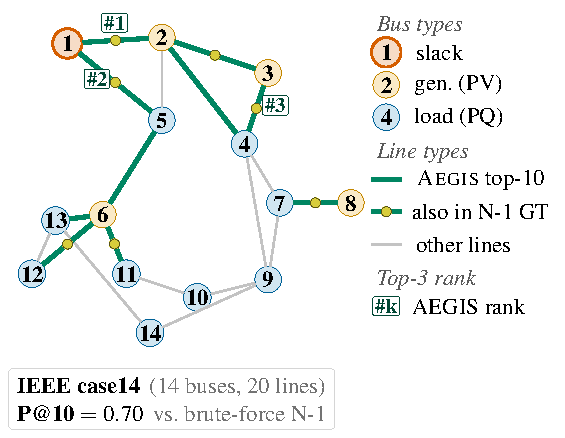
\includegraphics[width=0.92\columnwidth]{figures/fig_ieee14_case.pdf}
\caption{\AEGIS vulnerability ranking on the IEEE 14-bus benchmark (10-seed mean; P@10 $= 0.70$ for this run, consistent with the $0.74 \pm 0.12$ in \cref{tab:ieee}). Bus markers encode physical bus type (slack / generator / load); green edges are the top-10 by $v_{ij}$ with rank tags ($\#1$--$\#3$); yellow midpoint dots mark edges that also appear in the brute-force N-1 top-10 ($7$ of $10$). Top-ranked edges concentrate on the high-flow inter-area tie lines (1--2, 1--5, 7--8), recovering the single-contingency severity pattern from one matrix-free SVD pass.}
\label{fig:ieee14_case}
\end{figure}

\textbf{Baselines and stability.} On the voltage-angle ground truth, LODF (industry DC screening) attains $\tau{=}0.44$--$0.58$ on credible cases, behind \AEGIS's $0.62$--$0.67$ on case57/118 (Wilcoxon $p{<}0.01$, overlap on case14/30); LODF retargeted to thermal-overload reaches $\mathrm{P@10}{=}0.60$ on case57. Ejebe--Wollenberg PI~\cite{ejebe1979automatic} ($n{=}2$): $\tau{=}{+}0.335,\mathrm{P@10}{=}0.50$ on case57; $+0.101,0.30$ on case118. PTDF standalone (no outage correction) is anti-correlated on case57 ($\tau{=}{-}0.14$) and near-zero on case118 ($+0.06$), confirming outage redistribution is the operative effect. Runtime: LODF ${<}0.13$\,s; N-1 $0.1$--$2$\,s; \AEGIS $2$--$23$\,s. $v_1$ already recovers $40$--$64\%$ of N-2 critical sets via top-5 overlap from a one-query N-1-targeted pass, with pairwise rank stability $+0.40$--$+0.78$. \emph{Binary adjacency beats admittance-weighted} ($\mathrm{P@10}{=}0.81$ vs.\ $0.27$ on case118; Spearman admittance vs N-1 severity $-0.01$ to $+0.15$): a single-line trip removes the line regardless of impedance.
